\begin{mainquestion}{diode_001}{Diode Circuit}
Consider the circuit shown below:

\begin{center}
    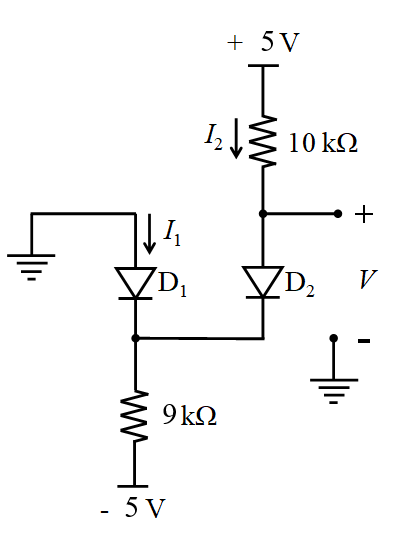
\includegraphics[width=0.5\textwidth]{questionbank/diodes/diode_001/v0/circuit.png}
\end{center}

% =========================================================
\begin{partquestion}{ideal}
{Find the values of $I_1$, $I_2$, and $V$ assuming an ideal diode model.}

\begin{answer}
With two diodes, we can check \(2^2 = 4\) assumed diode states to find a valid solution.

\textbf{Let us first assume $D_1$ and $D_2$ are both off.} This would imply that $I_1$ and $I_2$ are both zero, and that the voltage at $D_2$'s cathode is higher than its anode—this is a contradiction since the cathode voltage would be \qty{-5}{\volt} and the anode voltage would be \qty{5}{\volt} with no current flow.

\textbf{Next we assume $D_1$ is on and $D_2$ is off.} This would imply that there is positive current flow through $D_1$, and that the voltage at $D_1$'s cathode is \qty{0}{\volt}. If $D_2$ is off, there should be no current $I_2$, and $D_2$'s anode would be \qty{5}{\volt}. This leads to a contradiction, since a \qty{5}{\volt} anode and a \qty{0}{\volt} cathode should be in the on state.

\textbf{Next we assume $D_1$ is off and $D_2$ is on.} This implies that the voltage at $D_1$'s cathode must be positive. However, if $D_2$ is on, $D_2$'s cathode and anode are at the same voltage. The resistance ladder formed with current $I_2$ has more voltage drop across the \qty{10}{\kilo\ohm} resistor than the \qty{9}{\kilo\ohm} resistor, and since the rails are symmetric about \(\pm\qty{5}{\volt}\), the cathode must be at a negative voltage, leading to a contradiction.

\textbf{Lastly, we assume $D_1$ and $D_2$ are both on.} The cathodes of $D_1$ and $D_2$ are at \qty{0}{\volt}. This implies that the current $I_2$ is

\[
I_2
=
\frac{\qty{5}{\volt}-\qty{0}{\volt}}
{\qty{10}{\kilo\ohm}}
=
\qty{0.5}{\milli\ampere}.
\]

and the current through the \qty{9}{\kilo\ohm} resistor is

\[
I_{\qty{9}{\kilo\ohm}}
=
\frac{\qty{0}{\volt}-\qty{-5}{\volt}}
{\qty{9}{\kilo\ohm}}
=
\qty{0.56}{\milli\ampere}.
\]

It follows from KCL that

\[
I_1
=
I_{\qty{9}{\kilo\ohm}}-I_2
=
0.56 - 0.5
=
\qty{0.06}{\milli\ampere}
\]

and we have a valid solution!
\end{answer}
\end{partquestion}

% =========================================================
\begin{partquestion}{drop}
{Repeat part (\cref{prob:diode_001:ideal}) using a constant voltage drop model with $V_D = \qty{0.7}{\volt}$.}

\begin{answer}
The process is much the same as part (a), but we must account for a \qty{0.7}{\volt} drop across the diode when in the forward bias regime, rather than \qty{0}{\volt} as in the ideal case.

\textbf{Let us first assume $D_1$ and $D_2$ are both off.} This would imply that $I_1$ and $I_2$ are both zero, and that the voltage across $D_2$ is less than \qty{0.7}{\volt}—this is a contradiction since the cathode voltage would be \qty{-5}{\volt} and the anode voltage would be \qty{5}{\volt} with no current flow.

\textbf{Next we assume $D_1$ is on and $D_2$ is off.} This would imply that there is positive current flow through $D_1$, and that the voltage at $D_1$'s cathode is \qty{-0.7}{\volt}. If $D_2$ is off, there should be no current $I_2$, and $D_2$'s anode would be \qty{5}{\volt}. This leads to a contradiction, since a \qty{5}{\volt} anode and a \qty{-0.7}{\volt} cathode should be in the on state.

\textbf{Next we assume $D_1$ is off and $D_2$ is on}. This implies that the voltage at $D_1$'s cathode must be greater than \qty{-0.7}{\volt}. If $D_2$ is on, $D_2$'s anode and cathode have a difference of \qty{0.7}{\volt}. Using KVL and Ohm's law we can write

\[
\qty{5}{\volt}
-
I_2\left(\qty{10}{\kilo\ohm}\right)
-
\qty{0.7}{\volt}
-
I_{\qty{9}{\kilo\ohm}}\left(\qty{9}{\kilo\ohm}\right)
-
\qty{-5}{\volt}
=
0
\]

Since $D_1$ is off, $I_{\qty{9}{\kilo\ohm}} = I_2$ and we can substitute into the above equation and simplify:

\[
\qty{9.3}{\volt}
-
I_2\left(\qty{19}{\kilo\ohm}\right)
=
0
\]

so

\[
I_2
=
\frac{\qty{9.3}{\volt}}{\qty{19}{\kilo\ohm}}
=
\qty{0.489}{\milli\ampere}
\qquad
I_1 = \qty{0}{\milli\ampere}
\]

It follows that

\[
V
=
5
-
I_2\left(\qty{10}{\kilo\ohm}\right)
=
5
-
(0.489)\left(10\right)
=
\qty{0.11}{\volt}.
\]

There is no contradiction here, so this is a valid solution.

For fun, we can check the last case—it better result in a contradiction! Assume $D_1$ and $D_2$ are both on. The cathodes of $D_1$ and $D_2$ are at \qty{-0.7}{\volt}, and the anode of $D_2$ is at \qty{0}{\volt} (just like $D_1$). This implies that

\[
I_2
=
\frac{\qty{5}{\volt}-\qty{0}{\volt}}
{\qty{10}{\kilo\ohm}}
=
\qty{0.5}{\milli\ampere}.
\]

The current through the \qty{9}{\kilo\ohm} resistor is

\[
I_{\qty{9}{\kilo\ohm}}
=
\frac{\qty{-0.7}{\volt}-\qty{-5}{\volt}}
{\qty{9}{\kilo\ohm}}
=
\qty{0.478}{\milli\ampere}.
\]

It follows from KCL that

\[
I_1
=
I_{\qty{9}{\kilo\ohm}}-I_2
=
0.478-0.5
=
\qty{-0.022}{\milli\ampere}.
\]

which is a contradiction, since we said $D_1$ should be on (and conducting positive current $I_1$!). All is well with our analysis!
\end{answer}
\end{partquestion}

% =========================================================
\begin{partquestion}{level}
{If you were to somehow lower the diode’s forward voltage below \qty{0.7}{\volt}, at what voltage level will the operating state of $D_1$ and/or $D_2$ first change?}

\begin{answer}
We can use the extra work we did in the final state check for part (\cref{prob:diode_001:drop}) to see that we need to find the forward voltage drop that causes $I_1$ to just become non-negative. That occurs at

\[
I_1
=
I_{\qty{9}{\kilo\ohm}}
-
I_2
=
\frac{-V_D-\qty{-5}{\volt}}{\qty{9}{\kilo\ohm}}
-
\frac{\qty{5}{\volt}-\qty{0}{\volt}}{\qty{10}{\kilo\ohm}}
=
\qty{0}{\milli\ampere}
\]

Solving for $V_D$ gives

\[
V_D
=
\qty{5}{\volt}
-
\frac{\qty{9}{\kilo\ohm}}{\qty{10}{\kilo\ohm}}
\left(\qty{5}{\volt}\right)
=
\qty{0.5}{\volt}
\]
\end{answer}
\end{partquestion}

% =========================================================
\begin{partquestion}{symbolic}
{Replacing the \qty{2}{\kilo\ohm} resistor with a generic $R_1$, the \qty{1.8}{\kilo\ohm} resistor with a generic $R_2$ and the $\pm\qty{3}{\volt}$ DC power supplies with a generic $\pm V_{\text{CC}}$, find the expression for $V_D$ that answers part (\cref{prob:diode_001:level}) above.}
\begin{answer}
This is actually just a more generic analysis of the previous step in part (\cref{prob:diode_001:drop}). Here we have

\[
I_1
=
I_{R2}
-
I_2
=
\frac{-V_D-(-V_{\text{CC}})}{R_2}
-
\frac{V_{\text{CC}}-\qty{0}{\volt}}{R_1}
=
0
\]

Solving for $V_D$ gives

\[
V_D
=
V_{CC}
-
\frac{R_2}{R_1}\left(V_{\text{CC}}\right)
=
V_{CC}\left(1-\frac{R_2}{R_1}\right).
\]
\end{answer}
\end{partquestion}

\end{mainquestion}